%%% Hlavní soubor. Zde se definují základní parametry a odkazuje se na ostatní části. %%%

%% Verze pro jednostranný tisk:
% Okraje: levý 40mm, pravý 25mm, horní a dolní 25mm
% (ale pozor, LaTeX si sám přidává 1in)
\documentclass[12pt,a4paper]{report}
\setlength\textwidth{145mm}
\setlength\textheight{247mm}
\setlength\oddsidemargin{15mm}
\setlength\evensidemargin{15mm}
\setlength\topmargin{0mm}
\setlength\headsep{0mm}
\setlength\headheight{0mm}
% \openright zařídí, aby následující text začínal na pravé straně knihy
\let\openright=\clearpage

%% Pokud tiskneme oboustranně:
% \documentclass[12pt,a4paper,twoside,openright]{report}
% \setlength\textwidth{145mm}
% \setlength\textheight{247mm}
% \setlength\oddsidemargin{15mm}
% \setlength\evensidemargin{0mm}
% \setlength\topmargin{0mm}
% \setlength\headsep{0mm}
% \setlength\headheight{0mm}
% \let\openright=\cleardoublepage

%% Použité kódování znaků: obvykle latin2, cp1250 nebo utf8:
\usepackage[utf8]{inputenc}

%% Ostatní balíčky
\usepackage{graphicx}
\usepackage{amsthm}
\usepackage{subcaption}

%% Balíček hyperref, kterým jdou vyrábět klikací odkazy v PDF,
%% ale hlavně ho používáme k uložení metadat do PDF (včetně obsahu).
%% POZOR, nezapomeňte vyplnit jméno práce a autora.
\usepackage[unicode]{hyperref}   % Musí být za všemi ostatními balíčky
\hypersetup{pdftitle=Parallelization of Clustering Algorithms}
\hypersetup{pdfauthor=Bc. Jakub Vlček}

%%% Drobné úpravy stylu

% Tato makra přesvědčují mírně ošklivým trikem LaTeX, aby hlavičky kapitol
% sázel příčetněji a nevynechával nad nimi spoustu místa. Směle ignorujte.
\makeatletter
\def\@makechapterhead#1{
  {\parindent \z@ \raggedright \normalfont
   \Huge\bfseries \thechapter. #1
   \par\nobreak
   \vskip 20\p@
}}
\def\@makeschapterhead#1{
  {\parindent \z@ \raggedright \normalfont
   \Huge\bfseries #1
   \par\nobreak
   \vskip 20\p@
}}
\makeatother

% Toto makro definuje kapitolu, která není očíslovaná, ale je uvedena v obsahu.
\def\chapwithtoc#1{
\chapter*{#1}
\addcontentsline{toc}{chapter}{#1}
}

\begin{document}

% Trochu volnější nastavení dělení slov, než je default.
\lefthyphenmin=2
\righthyphenmin=2

%%% Titulní strana práce

\pagestyle{empty}
\begin{center}

\large

Charles University in Prague

\medskip

Faculty of Mathematics and Physics

\vfill

{\bf\Large MASTER THESIS}

\vfill

\centerline{\mbox{\includegraphics[width=60mm]{img/logo.eps}}}

\vfill
\vspace{5mm}

{\LARGE Bc. Jakub Vlček}

\vspace{15mm}

% Název práce přesně podle zadání
{\LARGE\bfseries Parallelization of Clustering Algorithms}

\vfill

% Název katedry nebo ústavu, kde byla práce oficiálně zadána
% (dle Organizační struktury MFF UK)
Department of Software Engineering

\vfill

\begin{tabular}{rl}

Supervisor of the master thesis: & RNDr. Martin Kruliš, Ph.D. \\
\noalign{\vspace{2mm}}
Study programme: & Informatics \\
\noalign{\vspace{2mm}}
Specialization: & Software Systems \\
\end{tabular}

\vfill

% Zde doplňte rok
Prague 2015

\end{center}

\newpage

%%% Následuje vevázaný list -- kopie podepsaného "Zadání diplomové práce".
%%% Toto zadání NENÍ součástí elektronické verze práce, nescanovat.

%%% Na tomto místě mohou být napsána případná poděkování (vedoucímu práce,
%%% konzultantovi, tomu, kdo zapůjčil software, literaturu apod.)

\openright

\noindent
Dedication.

\newpage

%%% Strana s čestným prohlášením k diplomové práci

\vglue 0pt plus 1fill

\noindent
I declare that I carried out this master thesis independently, and only with the cited
sources, literature and other professional sources.

\medskip\noindent
I understand that my work relates to the rights and obligations under the Act No.
121/2000 Coll., the Copyright Act, as amended, in particular the fact that the Charles
University in Prague has the right to conclude a license agreement on the use of this
work as a school work pursuant to Section 60 paragraph 1 of the Copyright Act.

\vspace{10mm}

\hbox{\hbox to 0.5\hsize{%
In ........ date ............
\hss}\hbox to 0.5\hsize{%
Jakub Vlček
\hss}}

\vspace{20mm}
\newpage

%%% Povinná informační strana diplomové práce

\vbox to 0.5\vsize{
\setlength\parindent{0mm}
\setlength\parskip{5mm}

Název práce:
Parallelization of Clustering Algorithms
% přesně dle zadání

Autor:
Bc. Jakub Vlček

Katedra:  % Případně Ústav:
Katedra softwarového inženýrství 
% dle Organizační struktury MFF UK

Vedoucí diplomové práce:
RNDr. Martin Kruliš, Ph.D., Katedra softwarového inženýrství 
% dle Organizační struktury MFF UK, případně plný název pracoviště mimo MFF UK

Abstrakt:
V diplomové práci se zabývám využitím moderních procesorových architektur, zvláště pak grafických čipů, k paralelizaci náročných výpočetních problémů, jakým je například shluková analýza. Na tomto problému zkoumám možnosti zrychlení na různých typech architektur (CPU a GPU) a především závislosti různých vstupních dat a různých přístupů k paralelizaci. Ty se odvíjí například od počtu vlastností (dimenze), které zkoumané objekty mají. Dále je také v práci dbáno na co nejefektivnější využití daných architektur (propustnost paměti, využití co nejvyššího počtu jader, minimalizace závislostí), kde není problém pouze rozdíl mezi CPU a GPU, ale i v jednotlivých verzích konkrétní architektury.
% abstrakt v rozsahu 80-200 slov; nejedná se však o opis zadání diplomové práce

Klíčová slova:
dolování dat, shluková analýza, paralelizace, GPU, CUDA
% 3 až 5 klíčových slov

\vss}\nobreak\vbox to 0.49\vsize{
\setlength\parindent{0mm}
\setlength\parskip{5mm}

Title: Parallelization of Clustering Algorithms
% přesný překlad názvu práce v angličtině

Author:
Bc. Jakub Vlček

Department:
Department of Software Engineering
% dle Organizační struktury MFF UK v angličtině

Supervisor:
RNDr. Martin Kruliš, Ph.D., Department of Software Engineering
% dle Organizační struktury MFF UK, případně plný název pracoviště
% mimo MFF UK v angličtině

Abstract:
The thesis deals with the use of the newest processor architectures, especially graphics processors (GPU), for parallelization of sophisticated computational problems such as cluster analysis. On this problem, I investigate possibilities of speed-up different types of architectures (CPU and GPU) and especially the dependence of different input data and different approaches to parallelization. For example, problem is the diversity of input data (the number of object properties). Furthermore, this thesis deals with on the most efficient use of the architecture like memory bandwidth, use the maximum number of cores, minimizing dependencies. Problem is not only in difference between CPU and GPU architecture but also in the different versions of a particular architecture.
% abstrakt v rozsahu 80-200 slov v angličtině; nejedná se však o překlad
% zadání diplomové práce

Keywords:
data mining, cluster analysis, parallelization, GPU, CUDA
% 3 až 5 klíčových slov v angličtině

\vss}

\newpage

%%% Strana s automaticky generovaným obsahem diplomové práce. U matematických
%%% prací je přípustné, aby seznam tabulek a zkratek, existují-li, byl umístěn
%%% na začátku práce, místo na jejím konci.

\openright
\pagestyle{plain}
\setcounter{page}{1}
\tableofcontents

%%% Jednotlivé kapitoly práce jsou pro přehlednost uloženy v samostatných souborech
\chapter{Introduction}

In this thesis, we deal with parallelization of speeding up cluster analysis and dependency between input data properties and different approaches to parallelization.
The main motivation for choosing this topic was not very widespread use of graphics cards whose performance with each generation increases rapidly. We want to use this potential to accelerate the current algorithmic problems, which are very compute-intensive. Such problems include the right cluster analysis, which has a very broad scope of application so it is very useful to accelerate it using the most modern hardware.

\section{Cluster Analysis} \label{sec:clusteranalysis}
Cluster analysis is a task that assigns a group to each object from the input set so that each group consists of objects with similar properties. Similar means that same property of two objects differs minimally in comparsion to same property of other objects. This means that each cluster contains objects that are more similar than objects from other groups. Hence the cluster analysis may be performed only on sets of objects of which must each be described by the same set of properties. This analysis has a wide range of applications, such as data mining, pattern recognition, machine learning, and many more.\\
Cluster analysis itself is only a task to be solved, not a concrete algorithm. There are many ways to solve this task, but they differ significantly in defining what cluster is and in cluster search efficiency. Most commonly definitions of the cluster are groups with small distances between the objects from the same cluster, dense areas of the input data, intervals or particular statistical distribution.\\
There are also two types of cluster organization. One way is hierarchically ordered clusters creates which creates a system of subsets where the intersection of the two is either the empty set or just one of them or non-hierarchical clusters, which creates system where clusters are disjoint sets. Because of complexity of the hierarchical clustering, in this thesis we deal with non-hierarchical type only.

\section{Cluster Models and Algorithms} \label{sec:clustermodels}
There are so many cluster models and one of the reasons why there exists a large amount of them is that the ``cluster'' cannot be precisely defined~\cite{EstivillCastro02}. Second reason is really wide applicability of this task so people from different departments approach this problem differently, because their notion of cluster differs significantly. \\

There exist many clustering algorithms because of many cluster models but there exist no universal algorithm, such an algorithm that covers all cluster models. Each algorithm was designed to cover one model or a subset of models and usually it is weak or not applicable for other models.\\
Because all of these algorithms counts distance, appropriate metric must be used. Some commonly used metric are:
\begin{description}
\item[Manhattan distance $L_1$] $$\|a-b\|_1=\sum_i |a_i - b_i| $$
\item[Euclidian distance $L_2$] $$\|a-b\|_2=\sqrt{\sum_i (a_i - b_i)^2 }$$
\item[Squared Euclidian distance $L_2^2$] $$\|a-b\|_2^2=\sum_i (a_i - b_i)^2 $$
\item[$p$-norm distance $L_p$] $$\|a-b\|_p=(\sum_i |a_i - b_i|^p)^\frac{1}{p} $$
\item[Maximum distance $L_\infty$] $$\|a-b\|_\infty=\lim_{p\to\infty}(\sum_i |a_i - b_i|^p)^\frac{1}{p}=\max_i |a_i - b_i| $$
\end{description}
All of these methods are only applicable for numeric data, so for other types, different metrics must be used (for example, Levenshtein for text, Mahalanobis for distance between point and distribution).
\\
The most typical models of clusters and algorithms are:
\begin{description}
\item[Well-Separated Clusters] Objects are well separated. Cluster is a set of objects such that each object in cluster is closer to objects from its cluster than to objects from other clusters~\autoref{fig:wellSeparatedObjects}. This is the easiest data input and most of algorithms performs well in this case.

\item[Center-Based Clusters] Object belongs to cluster if it is closer to the ``center'' of the cluster than ``centers'' of all other clusters.~\autoref{fig:centerBasedClusters} Center of cluster is usually called centroid or mean and it could represents whole cluster. This is good model for k-means like algorithms. \\
\textit{\textbf{Center-based clustering}} representing clusters as central object, which may not be part of the input data set.  For example \textit{\textbf{k-means}} algorithm takes $k$ centers and than each object is assigned to nearest center. Again, many metrics could be used, but commonly \textit{Euclidian distance} or \textit{Squared Euclidian distance} is used. \textit{\textbf{k-means}} clustering is basically an optimization problem where we looking for $k$ centers so distances will be the lowest possible. Problem is that optimization itself is NP-hard problem, so solution is commonly only approximate solution is searched. Approximation is commonly done by many iterations consist of assigning clusters to objects and  counting new means.
There are many variants of \textit{\textbf{k-means}} algorithm, they will be described later %TODO add ref too kmeans section
%\begin{description}
%\item[k-medoids] - centers are only objects from input data set
%\item[k-medians] - median is used instead of mean
%\item[k-means++] - initial centers are chosen randomly
%\item[Fuzzy k-means] - fuzzy cluster assignment is allowed
%\end{description}

One of the biggest problems of \textbf{k-means} algorithms is that the number of clusters must be specified at the beginning. Second problem is that clusters with similar size are used (in term of distance, not number of contained objects). This usually leads to splitting bigger clusters into smaller ones, because algorithm optimize cluster centers, not borders.
Output of \textit{\textbf{k-means}} like algorithms is usually input data set split in \textit{Voronoi cells}which could be useful for some problems.

\item[Contiguous Clusters] This model is similar to Center-Based Clusters model but there is difference that two clusters can merge into one. In other words, object is in cluster if it is similar to one ore more other objects from cluster.~\autoref{fig:contiguousClusters}\\
Main idea of \textbf{Contiguity-based clustering} is that objects that are nearby are more related than objects that are farther, so these algorithms grouping objects based on their distance only. Each cluster can be described by sum of distances or by maximum distance needed to connect objects in cluster. Having these cluster property, they can be easily ordered into hierarchy so parent clusters needs little more distance to connect its objects. This hierarchy could be represented as a dendrogram, which is tree diagram showing cluster hierarchy.\\

Other problem is the selection of linkage criterion, because cluster consists of many objects, there are many choices to compute the distance to. There are several methods for choosing linkage criteria between two sets of objects $A$ and $B$, $d$ is chosen metric:
\begin{description}
\item[Maximum or complete linkage clustering] $$\max\{d(a,b) : a \in A, b \in B\}$$
\item[Minimum or single linkage clustering] $$\min\{d(a,b) : a \in A, b \in B\}$$
\item[Mean or average linkage clustering, or UPGMA] (Unweighted Pair Group Method with Arithmetic Mean) $$\frac{1}{|A||B|}\sum_{a \in A} \sum_{b \in B} d(a,b)$$
\item[Centroid linkage clustering, or UPGMC] (Unweighted Pair-Group Method using Centroids) $$\|c_a - c_b\| \mbox{ where } c_a \mbox{ and } c_b \mbox{ are the centroids of clusters } A \mbox{ and } B$$
\item[Minimum energy clustering] $$\frac{2}{nm}\sum_{i,j=1}^{n,m}\|a_i-b_j\|_2-\frac{1}{n^2}\sum_{i,j=1}^{n}\|a_i-a_j\|_2-\frac{1}{m^2}\sum_{i,j=1}^{m}\|b_{i}-b_{j}\|_{2}$$
\end{description}

These methods are not resistive for extreme objects, which cause generating new clusters or even merging others. These methods has generally $O(n^3)$ complexity so they are slow for large amount of data. There exist optimization for special cases which has only complexity $O(n^2)$. These methods are taken as obsolete.

\item[Density-Based Clusters] Clusters are dense regions of objects. They are separated by low-density regions. This method is useful when some noise is present because the low-density regions will cover them and clusters will not change.~\autoref{fig:densityClusters} \\
Clusters in \textbf{Density-based clustering} are defined as areas with higher density of objects than in the rest of input data. Standalone objects are taken as noise. One of the most popular method is \textit{DBSCAN}. It is similar to contiguity-based clustering, because it connecting points based on the distance, but it only connects points satisfying density criterion. This means that in neighborhood specified by distance must be a minimum number of objects. These objects are called core objects and form the basis of cluster. Than objects which do not satisfy the density criterion but are close enough to at least one point from the cluster are added to cluster too.\\
The advantage of this method is its computational modesty, because it require only linear number of range queries. This method is deterministic so there is no need to tun it in iterations.
Drawback of these methods is the $\epsilon$ density parameter so borders of clusters with smaller density could be interpreted as  noise. Also separating nearby clusters may cause problems to these methods.

\item[Distribution models] Clusters in distribution models are objects that belong to same probability distribution. It is possible that one object belongs to more clusters.\\
In \textbf{Distribution-based clustering}, clusters are defined as objects from the same or similar distribution. This approach basically emulates process of generating the input data and try to reconstruct the lost statistical parameters. Main problem of this typ of clustering is problem known as \textit{overfitting}. This means that more complex model is described by less complex one and the difference between them is marked as deviation or noise. For example 3 points from the neighborhood of parabola vertex will be described by linear function.\\
One of methods used in distribution-based clustering is \textit{Gaussian mixture models} where algorithm iteratively optimizing parameters of fixed number of Gaussian distributions.
Problem is that this method assuming Gaussian distributed data set, but this set may not have even a model.

\item[Conceptual Clusters] Objects in cluster has some properties same or similar, but other properties could differ significantly.~\autoref{fig:conceptualClusters}\\
As algorithm for Conceptual Clusters, we can use algorithm depends on other model properties and less significant properties of objects could be easily omitted.

\item[Graph-Based Models] For example cliques in graphs should represent clusters. Clique is subset of nodes where every two nodes are connected with edge.~\autoref{fig:graphClusters}\\
Because of special demands of this model, special algorithms are needed so we could use graph algorithms, for example Bron-Kerbosch algorithm for finding cliques. %TODO source!
\end{description}

\begin{figure}[h]
\centering
\begin{subfigure}{.5\textwidth}
  \centering
  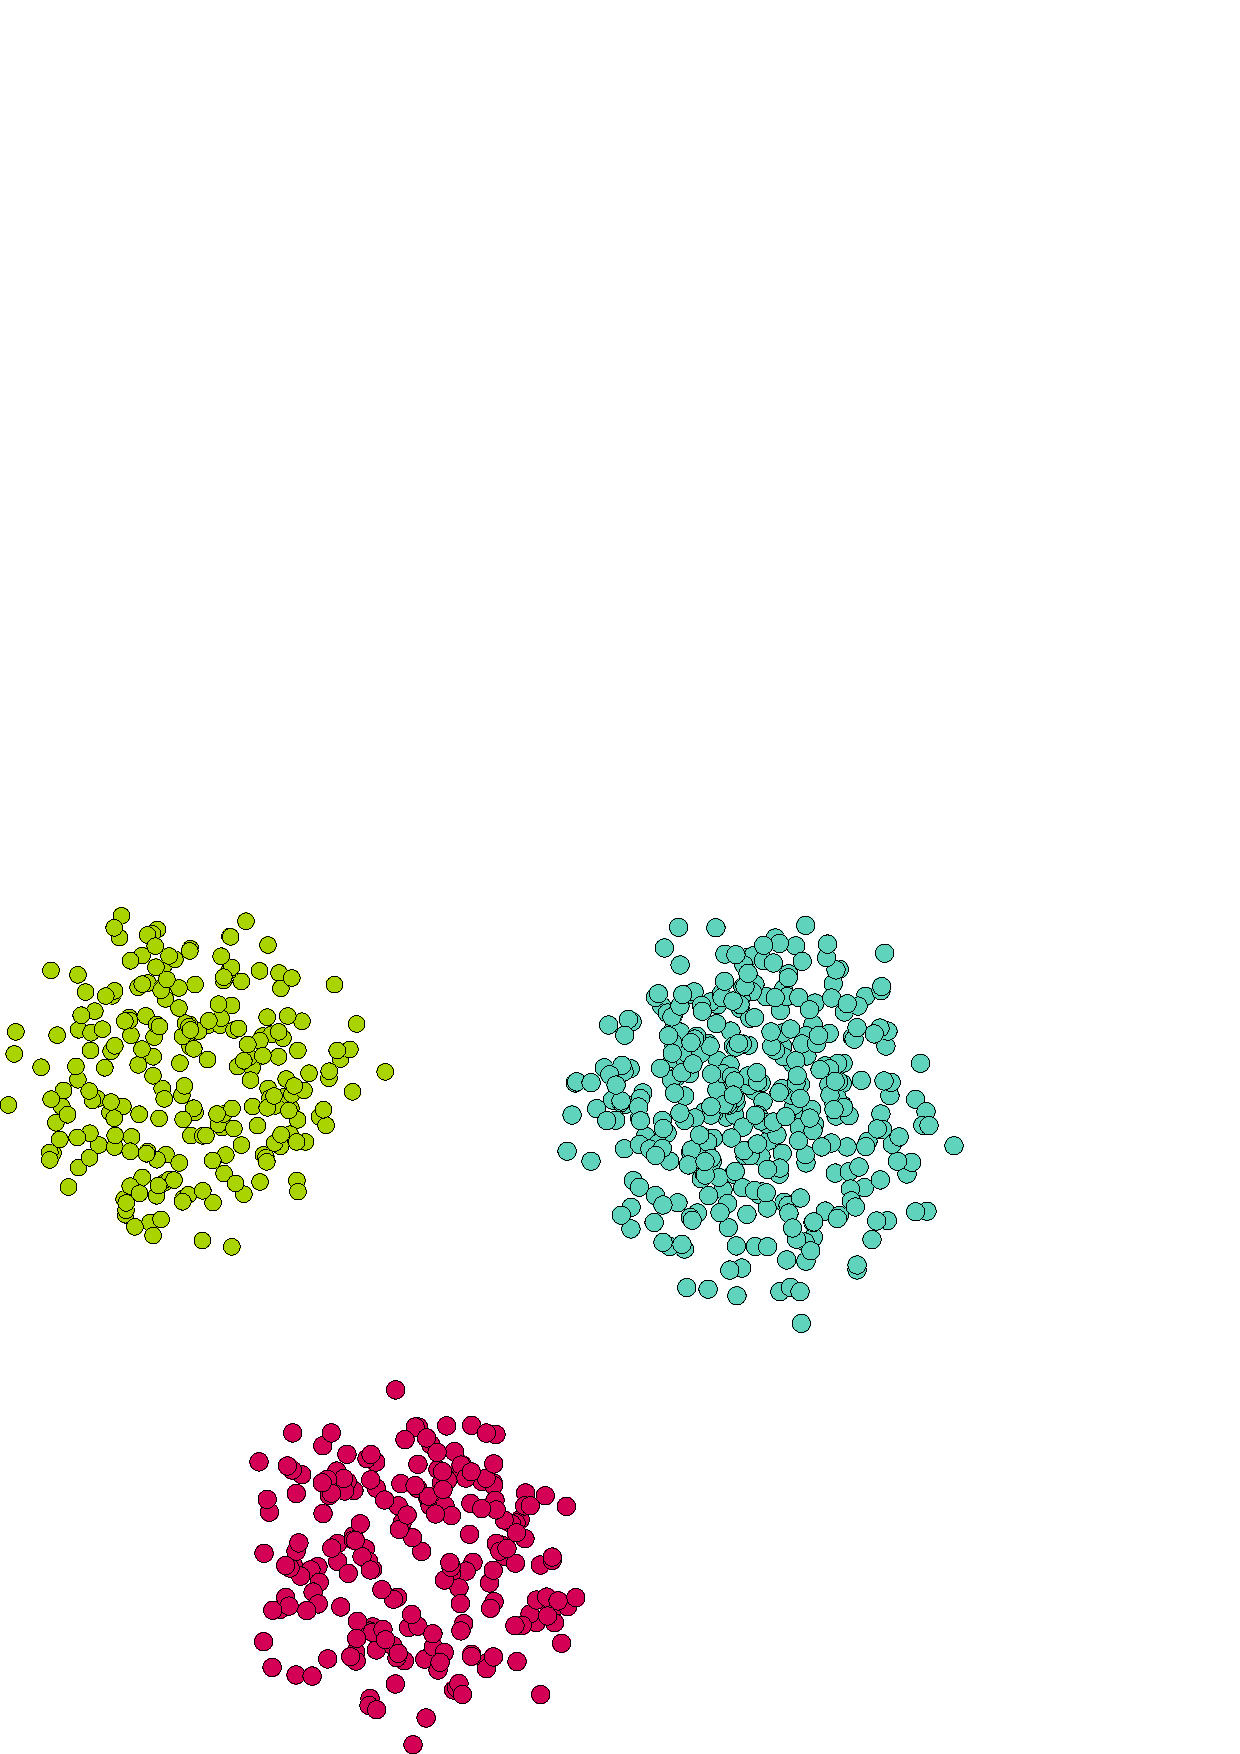
\includegraphics[width=.5\linewidth]{img/wellSeparatedObjects.png}
  \caption{Well sepatated objects}
  \label{fig:wellSeparatedObjects}
\end{subfigure}%
\begin{subfigure}{.5\textwidth}
  \centering
  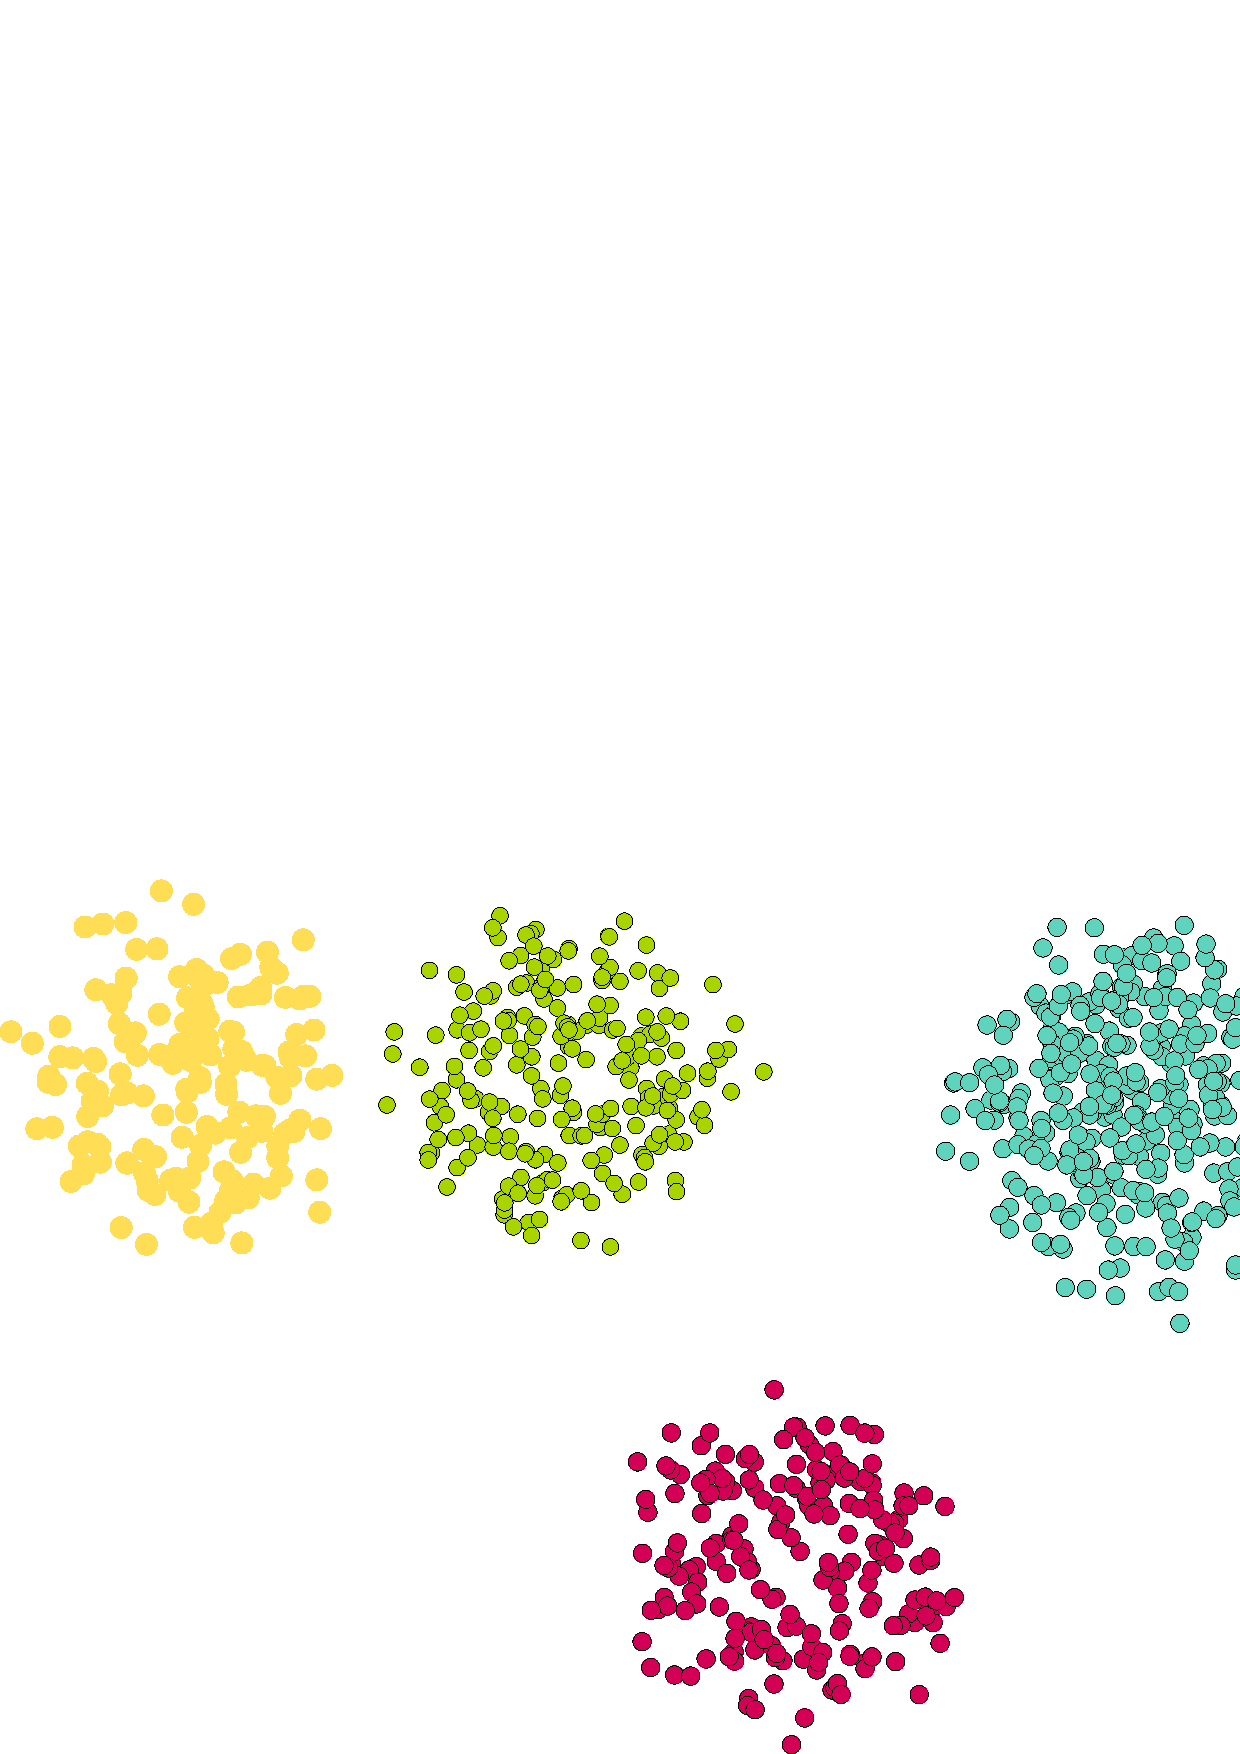
\includegraphics[width=.5\linewidth]{img/centerBasedClusters.png}
  \caption{Center-Based Clusters}
  \label{fig:centerBasedClusters}
\end{subfigure}%
\vspace*{0.5cm} 
\begin{subfigure}{.5\textwidth}
  \centering
  
\includegraphics[width=.5\linewidth]{img/contiguousClusters.png}
  \caption{Contiguous Clusters}
  \label{fig:contiguousClusters}
\end{subfigure}%
\begin{subfigure}{.5\textwidth}
  \centering
  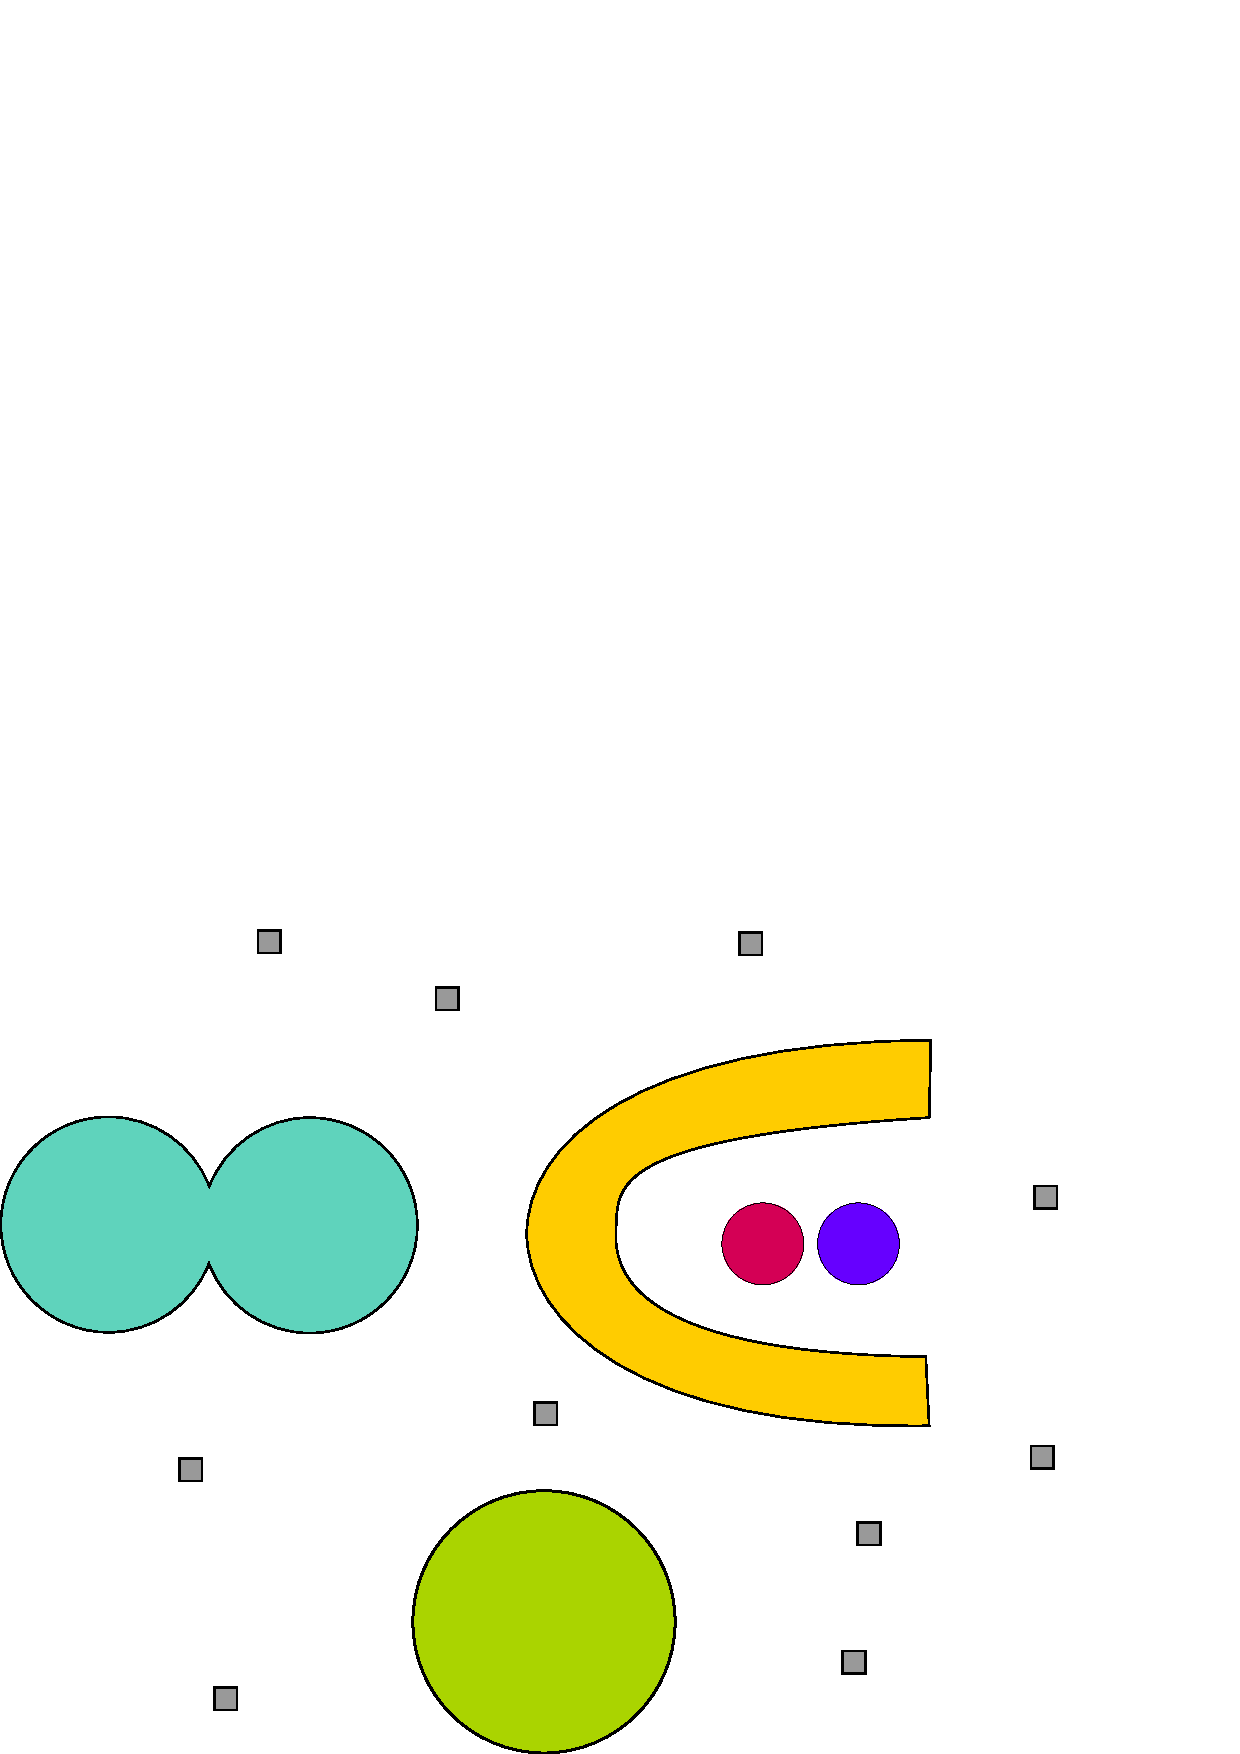
\includegraphics[width=.5\linewidth]{img/densityClusters.png}
  \caption{Density-Based Clusters (Gray squares represent noise)}
  \label{fig:densityClusters}
\end{subfigure}%
\vspace*{0.5cm} 
\begin{subfigure}{.5\textwidth}
  \centering
  \includegraphics[width=.5\linewidth]{img/conceptualClusters.png}
  \caption{Conceptual Clusters (Points in cluster have y-coordinate from specific range, omitting x-coordinate)}
  \label{fig:conceptualClusters}
\end{subfigure}%
\begin{subfigure}{.5\textwidth}
  \centering
  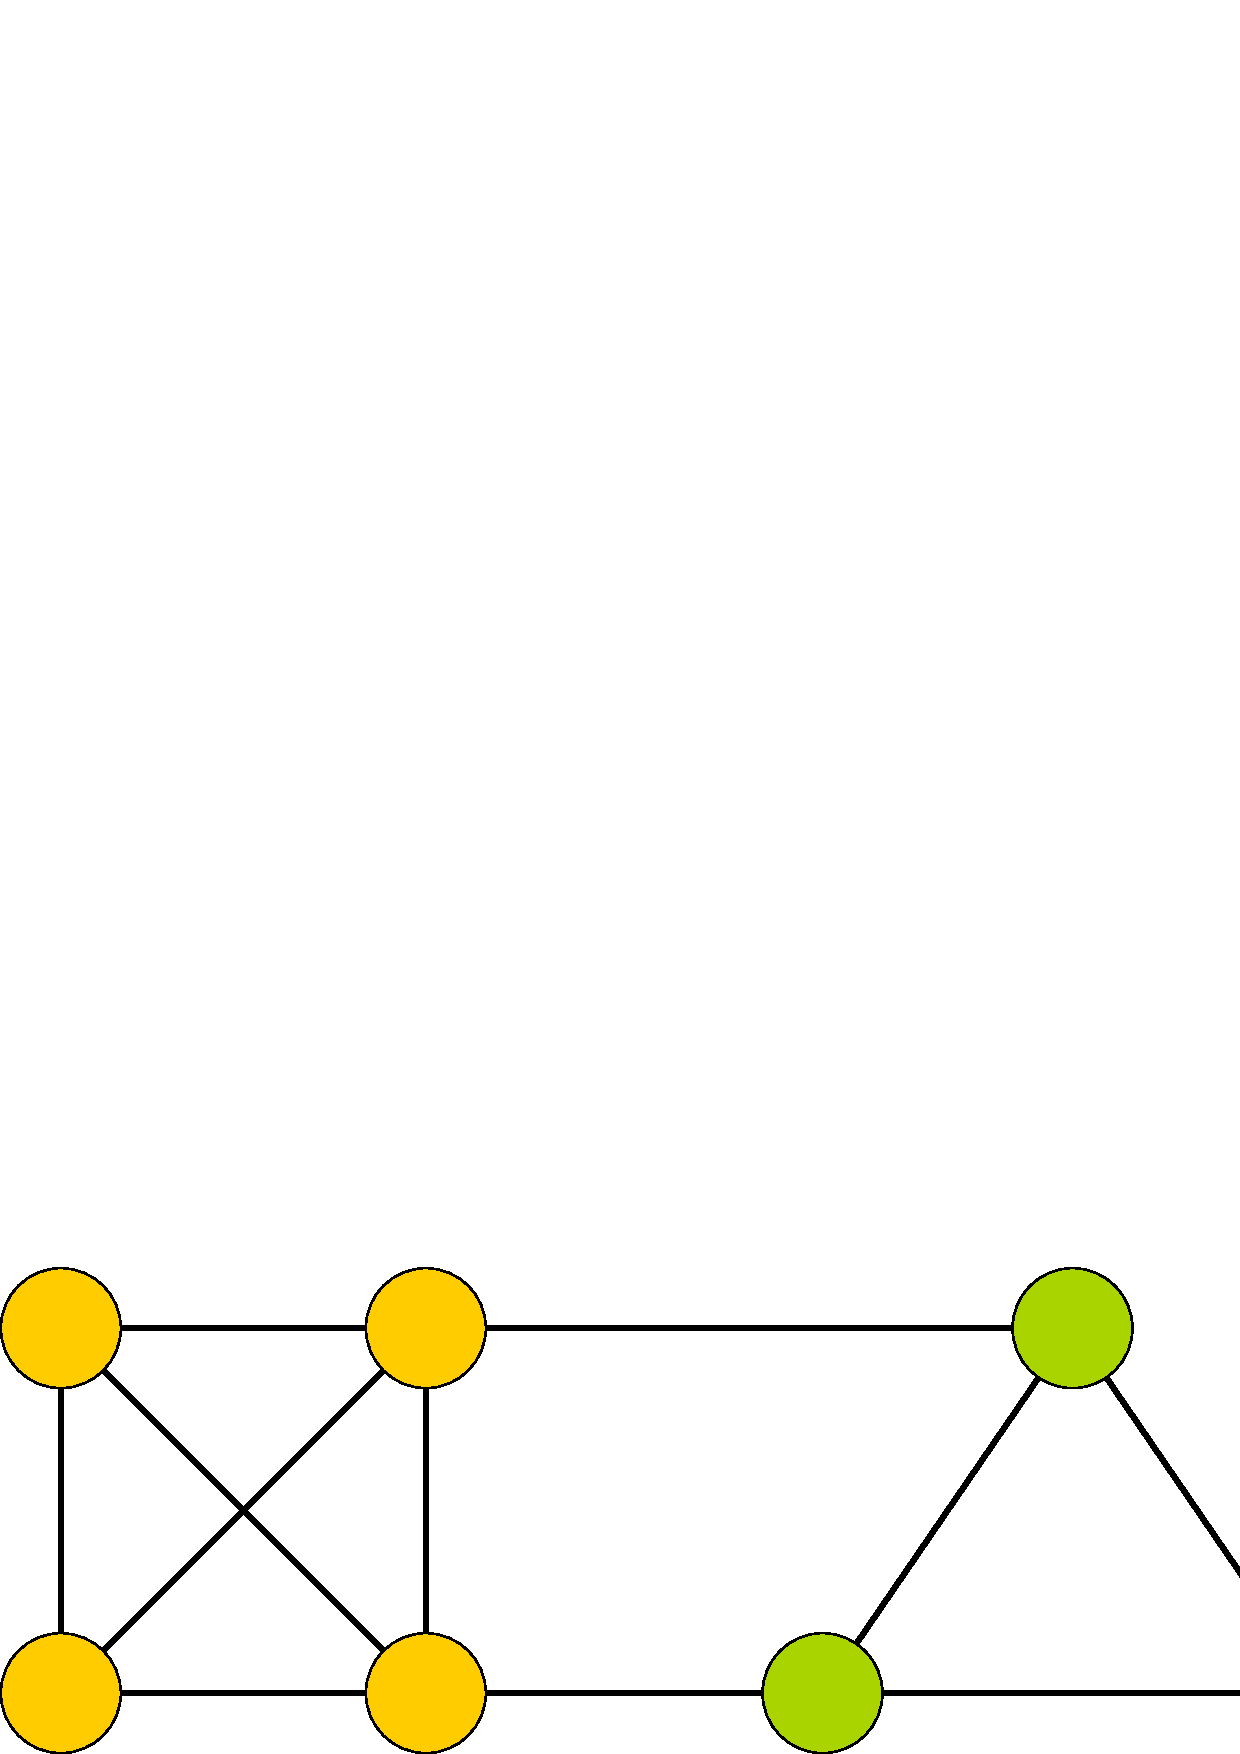
\includegraphics[width=.5\linewidth]{img/graphClusters.png}
  \caption{Graph-Based Clusters}
  \label{fig:graphClusters}
\end{subfigure}%
\caption{Typical cluster models}
\end{figure}

We can also divide clustering algorithms by relationship type:

\begin{description}
\item[Strict partitioning clustering] Objects belongs exactly into one cluster
\item[Strict partitioning clustering with outliers] Same as \textit{\textbf{strict partitioning clustering}} but object can be also unassigned. 
\item[Overlapping clustering] Object may belong to multiple clusters and we can specify, how much object belong to each cluster for example in percent.
\item[Hierarchical clustering] Object belongs also into parent clusters.
\end{description}

\section{Clustering Algorithms} \label{sec:clusteringAlgorithms}
 
\section{GPU parallelization}
\subsection{Compute Unified Device Architecture (CUDA)}
\chapter{Implementation}
\section{Platform}
We choose a C++ language for implementing our solutions, because we need low level code optimization and features like SIMD instructions, which are not available in other languages. Even if the CUDA is developed to work with multiple languages, cooperation with  C++ is one of the best, because also CUDA kernels are written in C++. Also platform independence of C++ is useful because we developed programs on Windows and than run on Linux clusters.

\section{K-means algorithm} \label{sec:kMeansAlgorithm}

As we can see in serial implementation~\autoref{lst:kMeansCode}, there are many cycles dependent on data size, so with growing number of data, serial version comes much slower. For example in two nested cycles on lines \autoref{lst:nestedCyclesBegin}-\autoref{lst:nestedCyclesEnd} of \autoref{lst:kMeansCode}, slowdown is great and this part of code is good target for parallelization.\\

\begin{lstlisting}[caption={k-means algorithm}, language=C++, escapeinside={\%*}{*)}, label={lst:kMeansCode}, numbers=left]
CreateLSH(width, hashTablesCount, basicHashFunctions)
{
  // Main iteration loop
  for( i = 0; i < iterationsCount; i++)
  {
    assign_to_clusters(data, means);
    compute_means(data_means);
  }
}

// Assign points to clusters
%*\label{lst:assignToClusters}*)assign_to_clusters(data, means)
{
//Iterate through data
%*\label{lst:nestedCyclesBegin}*)  for( d = 0; d < data_size; d++)
  {
    assigned_cluster = 0;
    min_distance = MAX_VALUE;
// Iterate through means
    for( m = 0; m < means_size; m++)
    {
      distance = count_distance( data[d], means[m] );
// If m-cluster is closer, reassign cluster
      if ( distance < min_distance )
      {
        assigned_cluster = m;
        min_distance = distance;
      }
    }
    data[d]->assigned_cluster = assigned_cluster;
%*\label{lst:nestedCyclesEnd}*)  }
}

// Compute new means
%*\label{lst:computeNewMeans}*)compute_means(data, means)
{
// Create new means array, all values are set to 0
  for( m = 0; m < means_size; m++)
  {
    new_means.push_back(new mean(0));
  }
  
// Iterate through data and accumulate data in appropriate new mean
  for( d = 0; d < data_size; d++)
  {
    assigned_cluster = data[d]->assigned_cluster;
    new_means[assigned_cluster]->contained_points++;
    for( dim = 0; dim < dimensions; dim++)
    {
      new_means[assigned_cluster]->coordinates[dim] +=
        data[d]->coordinates[dim];
    }
  }
  
// Count new means coordinates (arithmetic mean)
  for( m = 0; m < means_size; m++)
  {
    for( dim = 0; dim < dimensions; dim++)
    {
      new_means[m]->coordinates[dim] /=
        new_means[m]->contained_points;
    }
  }
}

// Function for counting distance
count_distance(point, mean)
{
  sum_squares = 0;
  for( dim = 0; dim < dimensions; dim++)
  {
    difference = point->coordinates[dim] - mean->coordinates[dim];
    sum_squares += difference * difference;
  }
  return sqrt( sum_squares );
}
\end{lstlisting}

\section{Parallelization}
As we mentioned in \autoref{sec:kMeansAlgorithm}, classical k-means algorithm contains many compute-intensive cycles, which could be parallelized. Problem is that the algorithm contains some compute dependencies, for example parallelization of nested cycles on lines \autoref{lst:nestedCyclesBegin}-\autoref{lst:nestedCyclesEnd} of \autoref{lst:kMeansCode} is problematic, because we need to accumulate coordinates in shared variable. These dependencies must be solved some way for correct parallelization.

\subsection{CPU versions}
We tried to used the most modern technologies offered by the newest CPU architectures to speed up k-means algorithm by parallelization. We created two levels of parallelization, first based on thread level (using more logical cores on single CPU) and than vectorization level using SIMD instructions.

\subsubsection{Thread level parallelization}
For thread level parallelization, we choose Threading Building Blocks (TBB) library from Intel. This library offers algorithms and data structures for parallel programing using multi-core processors but relieve programmer from complications arising from the use of native threading packages and handling particular threads. Manual thread creation, execution, synchronization and termination is hidden by using by creating TBB tasks which are processed on individual cores dynamically by the library. Also efficient use of CPU caches is automated.\\
We reworked program so points are split in groups, each group forming one TBB task.\\
\begin{description}
\item[Assigning to clusters]The first part of algorithm, assigning to clusters~\autoref{lst:kMeansCode},~\autoref{lst:assignToClusters}, is not so problematic, because only write operation is assigning cluster to point. Each point is contained in one and only one TBB task, which is processed by single thread, so it could not be read or written from other threads.\\
Second possible solution is to split means into groups and parallelize algorithm by tasks containing means. This solution is significantly slower, because we must synchronize writing information to each point about assigned cluster. If we want to remember this information in means (by accumulating assigned points to each mean) we hit a problem, because after assigning point to mean, we could not know if other mean is not closer to processed point so this way o parallelization is too computationally intensive.\\
\item[Compute new means]The second part of the algorithm, counting new means~\autoref{lst:kMeansCode},~\autoref{lst:computeNewMeans}, is more problematic, because we approach means from different TBB tasks, so accumulating of coordinates must be synchronized. We solved this problem by local copy of means in each TBB task, so we avoided the collisions. For joining tasks, we used TBB reduce algorithm, when to tasks are joined, local arrays of means coordinate sums are correctly added.\\
Also in this part of algorithm exists second possible solution by approaching parallelization by splitting means. This is more compute intensive because in this solution, for each mean, we must iterate through all points and accumulate coordinates but in previous solution, we iterate only through points and than, we join single tasks which takes logarithmic time depends on number of tasks.
\end{description}
Because both tasks are parallelized by same approach (splitting points to tasks, not the means), we joined both steps into one~\autoref{fig:computeflow} and gain more speed up because of omitting one start and one finish of TBB parallel task which has big overhead.
\begin{figure}[h]
  \centering
  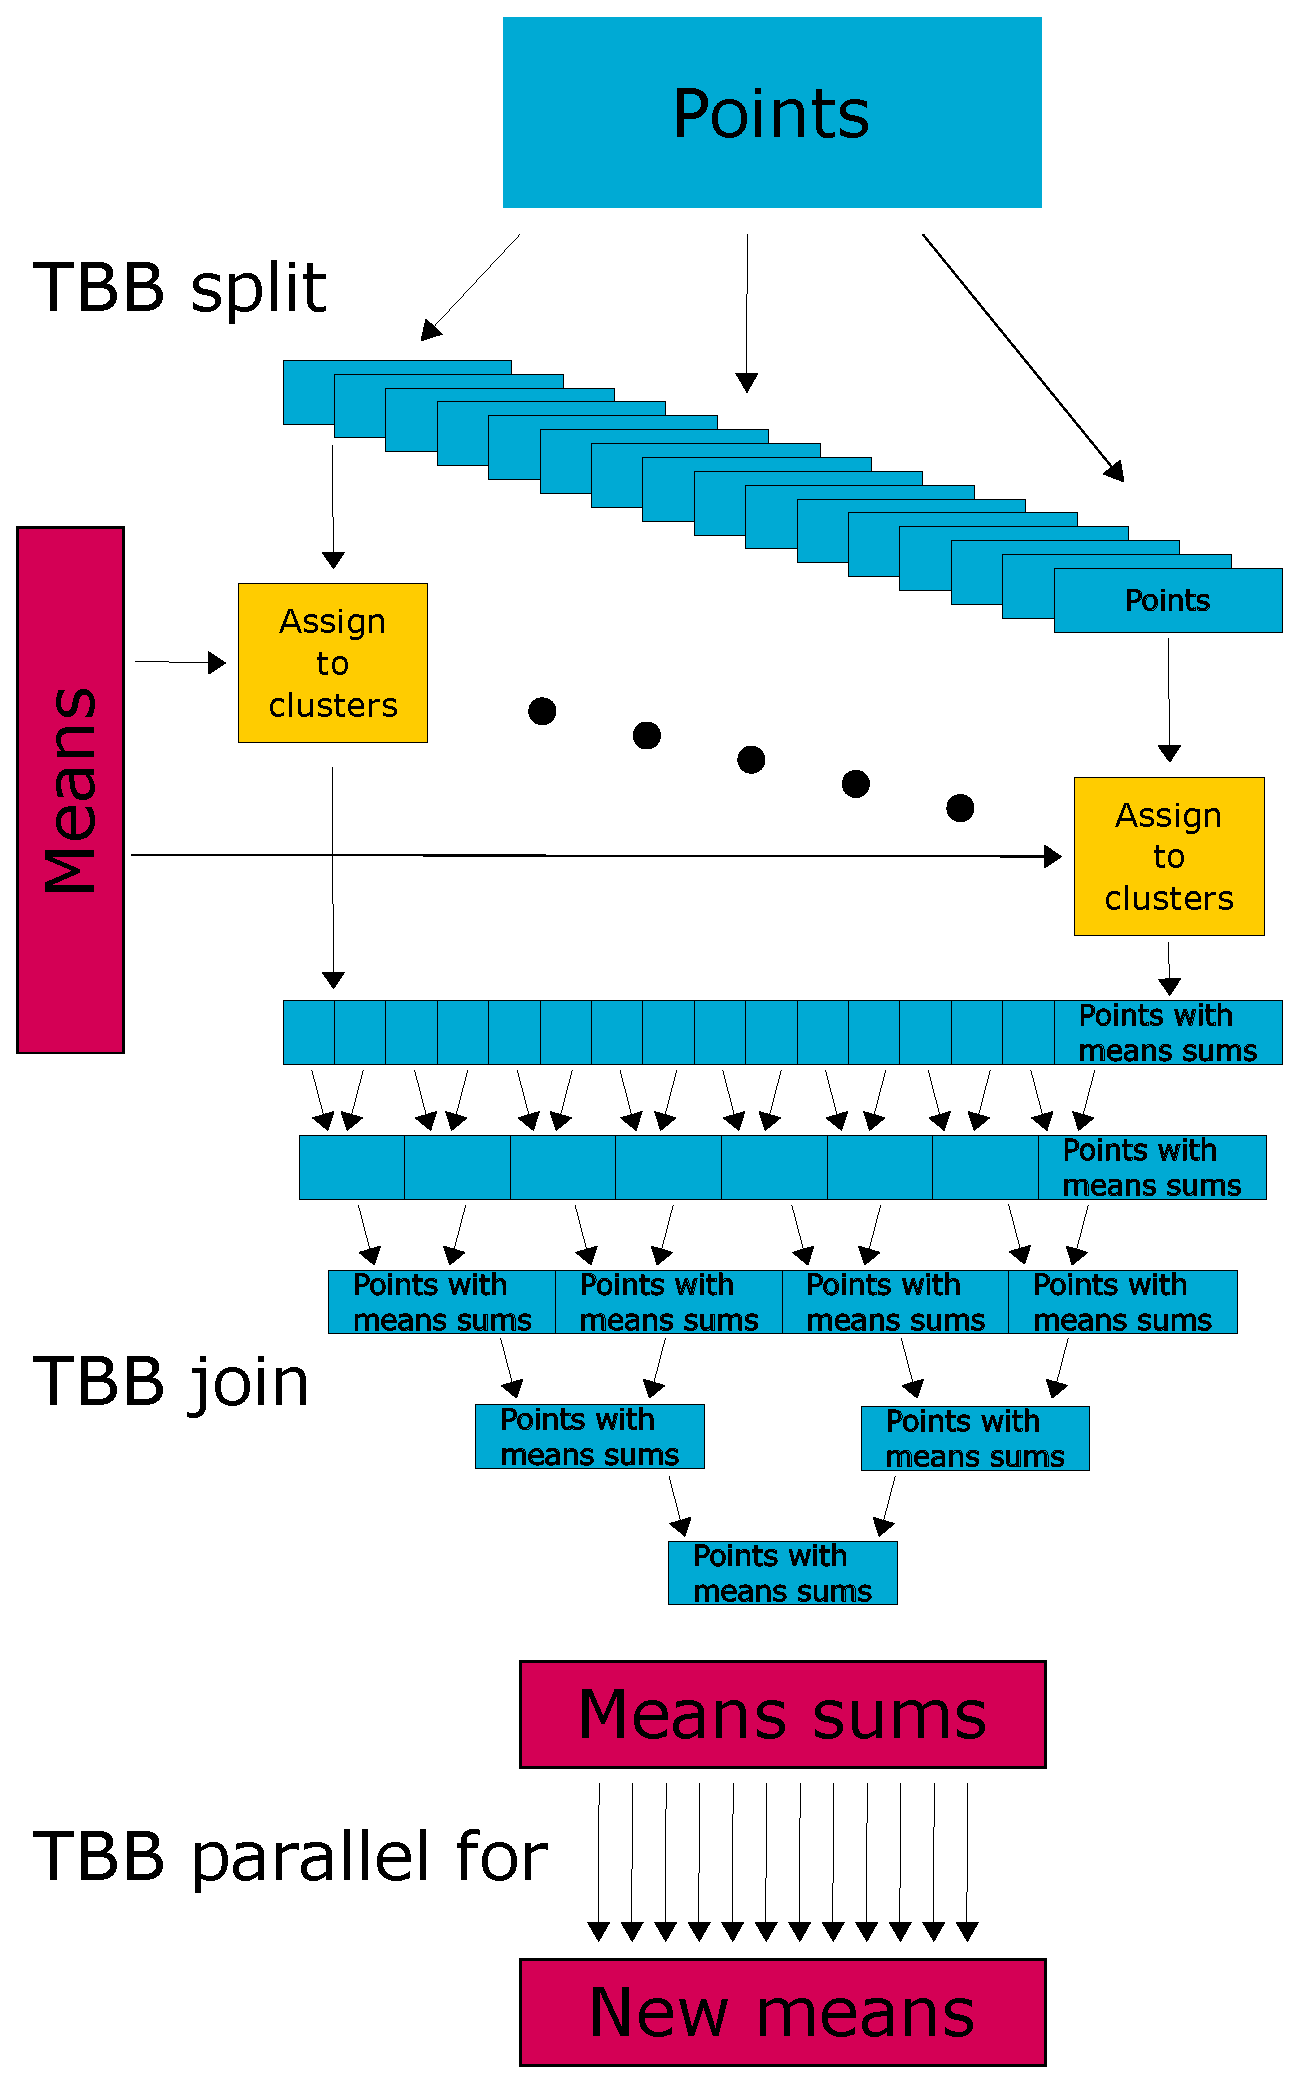
\includegraphics[width=1\linewidth]{img/computeFlow.eps}
  \caption{Compute flow}
  \label{fig:computeflow}
\end{figure}
\subsubsection{Vectorization}
For additional speed-up, we decided to use Simple instruction, multiple data (SIMD) as second layer of parallelization, concretely Streaming SIMD instructions (SSE), which are extension of x86 architecture. These instructions could greatly speed up the computation when exactly the same operations are performed on multiple data objects. Because points are already parallelized by TBB, we use SIMD inductions to parallelize smaller cycles iterating through dimensions, which are very often used in the algorithm. This cycle is usually much smaller (up to number of dimensions) than data but contains only few instructions which is precisely suitable for usage of SSE instructions so the loops will be up to four times faster (depend on number of dimensions) than non-SSE version.
\clearpage
\subsection{GPU versions}
For maximum speedup of this algorithm, we implemented versions using GPU, which offers hundreds of cores, so speed up of algorithm should be more than ten times better than parallel CPU version. Because of GPU architecture special features and the wide diversity of the input data, we developed more algorithm versions to reflect this particularities.\\
Also on GPU architecture we could divide algorithm to two layer of parallelization, using CUDA characteristics, because work on this platform is divided into blocks and each block is than executed by multiple threads. Because number of threads in single block is significantly bigger than possible count of instructions executed in parallel using SIMD, we decided to use different approach and use the thread layer in same way as the block layer, so both layers parallelize the task in terms of points.
Because the GPU compute effectiveness very depends on using different types of memory and the efficiency of its usage, it really depends on algorithm design. This problem is difficult to solve by single algorithm, because we need to use the data input characteristics. Here are some possibilities of data variety:
\begin{description}
\item[Big data] The first but maybe the biggest problem is the size of points. Because the input data are limited only by computer, so most often by host data storage, it can easily happen that the input data will not fit into the device biggest memory - global memory. Because this problem is also limiting on nonGPU versions, we have only focused on case when data fits in standardly the biggest memory on host - the RAM memory.
\item[Many dimensions] Other data problem could be many dimensions of the input space. Because basic GPU algorithm works similar as CPU version but without SIMD instructions, each thread in block must iterate through all dimensions which could be done better especially when the input data contains only few points.
\item[Few means] Opposite data attribute could be only few means. Than we could make several copies to fill in memory and avoid possible collisions. Problem is that we must join all copies onto so making so many copies is not so efficient.
\end{description}

The main problem is data size (both points and means) ín compare to memory size. In \autoref{tab:datamemoryfilling} is solution for each case when the appropriate data will not fit to the appropriate memory.

\newcolumntype{Y}{>{\RaggedRight\arraybackslash}X} 
\def\tabularxcolumn#1{m{#1}}
\begin{table}[h]
\centering
\caption{Data sizes and memory filling}
\label{tab:datamemoryfilling}
\begin{tabularx}{\textwidth}{|r|Y|Y|}
\cline{1-3}
\rowcolor[HTML]{AAD400} 
&Means&Points\\ \cline{1-3}
{\cellcolor[HTML]{AAD400}} Local memory&We could  share means between threads in Grid and store them in Shared memory.& Points are usually too bigger to fit in Local Memory, if so, we could place them into constant memory.\\ \cline{1-3}
{\cellcolor[HTML]{AAD400}} Shared memory&If means could not fit into Shared Memory, we could split them into more groups and make more iterations each only with means part.&Points sometimes could fit in Shared memory, if so, we could speed up the computation.\\ \cline{1-3}
{\cellcolor[HTML]{AAD400}} Global memory&If means does not fit even in Global memory on device, we must iterate through them, but this case usually does not occur.& When points are bigger than Global memory, we must swap appropriate part of them on device.\\ \cline{1-3}
\end{tabularx}
\end{table}

\subsubsection{Basic version}~\label{sssec:basicversion}
We have started with implementation of basic version, where we suppose that all data fits in device global memory. This implementation uses two CUDA kernels, first of them only find nearest cluster (\autoref{lst:findNearestClusterKernel} of \autoref{lst:simplekernel}). Each thread in block process one point by simple iterating through all means and dimensions. Number of threads in depends on SM capability of hardware. Number of blocks is simply the ceiling of number of points divided by number of threads per block. In this basic version, all data are stored in global memory and only memory caching is used for better memory latency. \\
Second task of this basic version is to count new means (\autoref{lst:countNewMeansKernel} of \autoref{lst:simplekernel}). In this kernel, each thread handles one mean. It iterates through all points and if point is assigned to appropriate mean, algorithm accumulates its coordinates. After all points are processed, new means are counted from accumulated sums by division by assigned points.\\
\\
\textcolor{red}{Add image with basic compute flow on CUDA?}
\\
\begin{lstlisting}[caption={CUDA simple kernel}, language=C++, escapeinside={\%*}{*)}, label={lst:simplekernel}, numbers=left]
%*\label{lst:findNearestClusterKernel}*)findNearestClusterKernel
  (meansSize, means[], dataSize, data[]
  , assignedClusters[], dimension)
{
  id = threadIdx.x + blockIdx.x * blockDim.x;
  minDistance = LLONG_MAX, distance = 0, difference = 0;
  for ( i = 0; i < meansSize; ++i )
  {
    distance = 0;
    for ( j = 0; j < dimension; ++j )
    {
      difference =
        means[ i * dimension + j ]
        - data[ id * dimension + j ];
      distance += difference * difference;
    }
    if (minDistance > distance)
    {
      minDistance = distance;
      assignedClusters[id] = i;
    }
  }
}


%*\label{lst:countNewMeansKernel}*)countNewMeansKernel
  (assignedClusters [], dataSize
  , data[], means[], dimension)
{
    id = threadIdx.x + blockIdx.x * blockDim.x;
    idOffset = id * dimension;
    count = 0;
    for ( i = idOffset; i < idOffset + dimension; ++i )
    {
        means[i] = 0;
    }
  %*\label{lst:bigdataloop}*)  for ( i = 0; i < dataSize; ++i )
    {
        if ( assignedClusters[i] == id )
        {
            for ( j = 0; j < dimension; ++j )
            {
                means[idOffset + j] +=
                  data[i * dimension + j];
            }
            ++count;
        }
    }
    for ( i = idOffset; i < idOffset + dimension; ++i )
    {
        means[i] /= count;
    }
}
\end{lstlisting}

\subsubsection{Atomic operations}
Because of huge slow down in the basic version~\autoref{sssec:basicversion} in counting new means from assigned clusters, we need to iterate through tens of thousands of points~(\autoref{lst:bigdataloop} in \autoref{lst:simplekernel})  and only if we hit point assigned to appropriate cluster, we accumulate its coordinates. This is because we could not accumulate these in find nearest cluster function (\autoref{lst:findNearestClusterKernel}), because we could get several race conditions when writing from many threads to single cluster. If we solved this problem, than second step of the algorithm could be only to divide accumulated coordinate sums by number of assigned cluster and avoid time-consuming loop through every point. This race conditions could be solved by atomic operations, which could easily protect accumulating of coordinates and avoid this problem, but atomic operations have some overhead and when we have only few means, this overhead causes a big algorithm slow down so in this case, this problem must be solved in some other way.

\subsubsection{Many dimensions problem}~\label{sssec:manyDims}
Because in basic version, each point is processed by single thread, kernel run could become slower when the dimension of input space is big. Like in CPU version with SIMD, we implemented a version which simulate SSE instructions so if the dimension of space is big enough, we launch thread block for each point and threads in these block works like SIMD and iterate through dimensions. Each thread has its local sum of distances in each dimension so than we need to add these values from each thread. Because these values must be accessible from all threads in warp, we used shared memory.\\
This could be solved by many ways so we tried to optimize this process for CUDA environment.\\
\\
\textcolor{red}{Add images of compute flow in each type of reduction?}
\\
\begin{description}
\item[Interleaved addressing] In this access, we reduce the partial sums in array of size $N$ iteratively. In each step, we need only half of a array from previous step, so in first step ($i=1$), we start $N/(i^2)$ threads, each thread access only partial sums on positions dividable by $2^i$, add partial sum from position $2^{(i-1)}$ bigger and store the value.
\begin{lstlisting}
for ( stride=1; stride < threadsInBlock; stride*=2)
{
  if (threadID % ( 2 * stride ) == 0)
  {
    sums[threadID] += sums[threadID + stride];
  }
  __syncthreads();
}
\end{lstlisting}
Main problem of this solution is that modulo operator is very slow and that in highly divergent warps, reduction is very inefficient.
\item[Interleaved addressing 2]This solution is similar to previous but we removed problems of first solution. At first, we removed the modulo operation and second thing is that in each we used only threads with IDs less than half of array size from previous step. 
\begin{lstlisting}
for ( stride=1; stride < threadsInBlock; stride*=2)
{  i = 2 * stride * threadID;
  if ( i < threadsInBlock)
  {
    sums[index] += sums[index + stride];
  }
  __syncthreads();
}
\end{lstlisting}
Because we using shared memory for sums, we hit a new problem, bank conflicts, so we must use little bit different approach if we need to solve this.
\item[Sequential addressing]Problem with bank conflicts could be solved by using reverse loop and different type of addressing. In this solution we used same threads as in previous solution, but we access only items on the front of the array. This means that we again start with half of threads than array size but each thread takes item from array with same id as thread id and sums it with item with id $threadID + stride$. This means that the actual partial sums in each step is in the front of the array so we have avoided bank conflicts.
\begin{lstlisting}
for ( stride=threadsInBlock; stride > 0; stride>>=1)
{
  if ( threadID < stride )
  {
    sums[threadID] += sums[threadID + stride];
  }
  __syncthreads();
}
\end{lstlisting}
Even in this solution we have problem with unused threads. In first iteration, half of them is unused, in second iteration, only a quarter of all threads working etc. This could be partially solved by making first step when loading data to share memory, so we need only half of all threads or in other words, we could process twice the data volume than without this improvement.
\item[Unrolling loop]Because we could select the number of threads in block, we could choose same number as number of cores in SM and because instructions are SIMD synchronous within warp, we do not need thread synchronization $syncthreads()$ and because we know the block size at the compile time, we could template this method so big part of work will be resolved in compile time.
\begin{lstlisting}
if (threadIdx.x < blockDim.x / 2)
  {
    if (blockSize >= 64) distances[threadId] +=
      distances[threadId + 32];
    if (blockSize >= 32) distances[threadId] +=
      distances[threadId + 16];
    if (blockSize >= 16) distances[threadId] +=
      distances[threadId + 8];
    if (blockSize >= 8) distances[threadId] +=
      distances[threadId + 4];
    if (blockSize >= 4) distances[threadId] +=
      distances[threadId + 2];
    if (blockSize >= 2) distances[threadId] +=
      distances[threadId + 1];
  }
\end{lstlisting}
\item[Shuffle instructions]From Compute capability 3.0, we could use special shuffle instructions. These instructions was designed for cooperation between threads in one warp and to thread process local data in warp scope. Usually when we need to exchange data between threads in warp, we are forced to use shared memory, because we can't access local memory from other thread and this is exactly what shuffle instructions resolving. When we use shuffle instructions, we could use only the local memory which is significantly lower latency and higher bandwidth than shared memory and in addition shuffle instructions are faster than instructions on shared memory - single instruction versus three on shared memory (write, synchronize, read). So when we use shuffle instructions for sum partial sums, we gain additional speed up (but only CC 3.0 and newer).
\end{description}

\subsubsection{Few means}
When we need to compute only few means, we could solve problems with conflicts by making local copies of all means sums in shared memory and than merge it in similar way as in~\autoref{sssec:manyDims}.\\
Each thread have its copy of means and shares it with only few other threads so we reduce conflicts by number of means copies. As an extreme case, every thread could have its own copy of means sums so we can completely avoid collisions. Problem is that we must merge all copies in next step, so we must select between number of collisions and merge demands.
Because merging of means copies is harder than merging distances (we don't merge all data into single value but we need to sum only corresponding data. Also the amount of data is many times bigger.\\
We also implemented solution for case when means closely do not fit in shared memory. Than we could split means and counts only with part of means and than compute the same task but with other part of means. Also this problem requires post processing because all points are assigned two more means (from each part we choose the nearest mean) so we need to choose the nearest means and than accumulate coordinates sums. Because post processing in this solution is harder, it makes sense only for small number of means parts.

\subsubsection{Big data}
Problem with big data is obvious because points could not fit in device memory. This could be solved by split data into smaller parts so we can fit two parts at once in global memory.Because on CUDA has capability to transfer data and process other data at once, we can work on one part which is already transfered on device while other chunk of points is transfered onto device.
Than we must compute new means but because we expect that means fit in device memory, we could use same function as in other solutions.

\section{??Tools??}
\subsection{??Data generation??}
\subsection{??Result validation??}
\chapter{Measurements and results}

\section{Measurements}

\section{Results}


% Ukázka použití některých konstrukcí LateXu (odkomentujte, chcete-li)
% \include{example}

\include{epilog}

%%% Seznam použité literatury
%%% Seznam použité literatury je zpracován podle platných standardů. Povinnou citační
%%% normou pro diplomovou práci je ISO 690. Jména časopisů lze uvádět zkráceně, ale jen
%%% v kodifikované podobě. Všechny použité zdroje a prameny musí být řádně citovány.

\def\bibname{Bibliography}
\begin{thebibliography}{99}
\addcontentsline{toc}{chapter}{\bibname}

%\bibitem{lamport94}
%  {\sc Lamport,} Leslie.
%  \emph{\LaTeX: A Document Preparation System}.
%  2. vydání.
%  Massachusetts: Addison Wesley, 1994.
%  ISBN 0-201-52983-1.

\bibitem{EstivillCastro02}
{\sc Estivill-Castro,} Vladimir
\emph{Why so many clustering algorithms.}
[online]. p.~65-75. DOI 10.1145/568574.568575.

\bibitem{Zechner09}
{\sc Zechner,} Mario, {\sc Granitzer, } Michael
\emph{Accelerating K-Means on the Graphics Processor via CUDA}
First International Conference on Intensive Applications and Services
2013
ISBN: 978-1466558212 

\bibitem{Aggarwal13}
{\sc Aggarwal,} Charu C., {\sc Reddy, } Chandan K.
\emph{Data Clustering: Algorithms and Applications}
Chapman \& Hall/CRC Data Mining and Knowledge Discovery Series
2009
ISBN: 978-1-4244-3683-5

\bibitem{Jain10}
{\sc Jain,} A.
\emph{Data clustering: 50 years beyond k-means}
Pattern Recognition Letters, 31(8):651–666
19th International Conference in Pattern Recognition (ICPR)
2010

\bibitem{Kaufman90}
{\sc JKaufman,} Leonard, {\sc Rousseeuw,} Peter J.
\emph{Finding Groups in Data: An Introduction to Cluster Analysis}
Wiley-Interscience
1990
ISBN: 978-0-4718-7876-6

\bibitem{Drineas04}
{\sc Drineas,} P., {\sc Frieze,} A., {\sc Kannan,} R., {\sc Vempala,}  S., {\sc Vinay,}  V.
\emph{Clustering large graphs via the singular value decomposition}
Machine Learning., 56(1-3):9–33.
2004
ISSN: 0885-6125

\bibitem{Bottou95}
{\sc Bottou,} L\'{e}on, {\sc Bengio,} Yoshua
\emph{Convergence Properties of the K-Means Algorithms}
Advances in Neural Information Processing Systems 7
p.~585-592
MIT Press, 1995

\bibitem{Kim14}
{\sc Kim,} Kyoungok
\emph{Voronoi Cell-Based Clustering Using a Kernel Support.}
Knowledge and Data Engineering, IEEE Transactions
ISSN: 1041-4347
DOI 10.1109/TKDE.2014.2359662. 

\bibitem{Vallender73}
{\sc Vallender,} S.S.
\emph{Calculation of the Wasserstein Distance Between Probability Distributions on the Line.}
[online]. s.~784--786. DOI: 10.1137/1118101.

\bibitem{Beecks10}
{\sc Beecks,} Christian, {\sc Uysal,} Merih Seran, {\sc Seidl,} Thomas
\emph{Signature Quadratic Form Distance.}
Proceedings of the ACM International Conference on Image and Video Retrieval - CIVR , 2010.
ACM
ISBN 978-1-4503-0117-6
DOI 10.1145/1816041.1816105

\bibitem{Tan05}
{\sc Tan,} Pang-Ning, {\sc Michael,} Steinbach, {\sc Kumar,} Vipin
\emph{Introduction to data mining.}
Pearson New International Edition
Boston: Pearson Addison Wesley, 2005
ISBN 978-0-3213-2136-7

\bibitem{Sun15}
{\sc Sun,} Xili, {\sc Tian,} Shoucai, {\sc Lu,} Yonggang
\emph{High dimensional data clustering by partitioning the hypergraphs using dense subgraph partition}
MIPPR 2015: Pattern Recognition and Computer Vision
DOI 10.1117/12.2205743.

\bibitem{Kirk12}
{\sc Kirk,}David B., {\sc Hwu}Wen-mei W.:
\emph{Programming Massively Parallel Processors}
Second Edition: A Hands-on Approach
2012
ISBN: 0124159923 

\bibitem{Sanders10}
{\sc Sanders,} Jason, {\sc Kandrot,} Edward
\emph{CUDA by Example: An Introduction to General-Purpose GPU Programming}
NVIDIA
2010
ISBN: 0-13-138768-5 

\bibitem{Scarpino11}
{\sc Scarpino,} Matthew
\emph{OpenCL in Action: How to Accelerate Graphics and Computations}
Manning Publications
2011
ISBN: 1617290173 

\bibitem{Hong09}
{\sc Bai,} Hong-Tao, {\sc He,} Li-li, {\sc Ouyang,} Dan-tong, {\sc Li,} Zhan-shan, {\sc Li, } He
\emph{K-means on commodity GPUs with CUDA}
 Computer Science and Information Engineering
 2009
 WRI World Congress on. Volume 3.
 IEEE (2009) 651–655 

\bibitem{CUDAGuide}
Nvidia
\emph{CUDA C PROGRAMMING GUIDE}
Nvidia, 2015
available online: http://docs.nvidia.com/cuda/cuda-c-programming-guide/
\end{thebibliography}

%%% Tabulky v diplomové práci, existují-li.
\chapwithtoc{List of Tables}

%%% Použité zkratky v diplomové práci, existují-li, včetně jejich vysvětlení.
\chapwithtoc{List of Abbreviations}

%%% Přílohy k diplomové práci, existují-li (různé dodatky jako výpisy programů,
%%% diagramy apod.). Každá příloha musí být alespoň jednou odkazována z vlastního
%%% textu práce. Přílohy se číslují.
\chapwithtoc{Attachments}

\openright
\end{document}
